\documentclass[10pt,a4paper]{article}
\renewcommand{\baselinestretch}{1.25}
%<---------------------------------------------------------------------------->%
%%% CJK %%%
\usepackage{xeCJK}
\newcommand{\chmainfont}{GenWanMin TJ L}
\newcommand{\chsansfont}{Noto Sans CJK KR Regular}
\newcommand{\chboldfont}{Noto Sans CJK KR Medium}
\newcommand{\chmonofont}{Noto Sans Mono CJK KR Regular}
\newcommand{\chitalfont}{LXGW WenKai Light}
\setCJKmainfont{\chmainfont}[BoldFont=\chboldfont,ItalicFont=\chitalfont]
\setCJKsansfont{\chsansfont}[BoldFont=\chboldfont]
\setCJKmonofont{\chmonofont}
\xeCJKsetup{PunctStyle=kaiming,CheckFullRight=true,CJKmath=true}
\setlength\parindent{2em}
%%% Punctuation width %%%
\xeCJKsetwidth{、}{0.55em}
\xeCJKsetwidth{,}{0.6em}
\xeCJKsetwidth{:}{0.65em}
\xeCJKsetwidth{;}{0.65em}
\xeCJKsetwidth{。}{0.7em}
\xeCJKsetwidth{・}{0.7em}
\xeCJKsetwidth{〈〉}{0.7em}
\xeCJKsetwidth{《》}{0.7em}
\xeCJKsetwidth{「」}{0.7em}
\xeCJKsetwidth{『』}{0.7em}
\xeCJKsetwidth{【】}{0.7em}
\xeCJKsetwidth{()}{0.7em}
%<--------------------------------------------------------------------------->%
%%% Punctuation Kerning %%%
% Pairs-with-punctuation kerning (after).
\xeCJKsetkern{〉}{、}{0.2em} \xeCJKsetkern{〉}{,}{0.2em} \xeCJKsetkern{〉}{。}{0.2em} \xeCJKsetkern{〉}{;}{0.2em} \xeCJKsetkern{〉}{:}{0.2em}
\xeCJKsetkern{》}{、}{0.2em} \xeCJKsetkern{》}{,}{0.2em} \xeCJKsetkern{》}{。}{0.2em} \xeCJKsetkern{》}{;}{0.2em} \xeCJKsetkern{》}{:}{0.2em}
\xeCJKsetkern{」}{、}{0.2em} \xeCJKsetkern{」}{,}{0.2em} \xeCJKsetkern{」}{。}{0.2em} \xeCJKsetkern{」}{;}{0.2em} \xeCJKsetkern{」}{:}{0.2em}
\xeCJKsetkern{』}{、}{0.2em} \xeCJKsetkern{』}{,}{0.2em} \xeCJKsetkern{』}{。}{0.2em} \xeCJKsetkern{』}{;}{0.2em} \xeCJKsetkern{』}{:}{0.2em}
\xeCJKsetkern{】}{、}{0.2em} \xeCJKsetkern{】}{,}{0.2em} \xeCJKsetkern{】}{。}{0.2em} \xeCJKsetkern{】}{;}{0.2em} \xeCJKsetkern{】}{:}{0.2em}
\xeCJKsetkern{)}{、}{0.2em} \xeCJKsetkern{)}{,}{0.2em} \xeCJKsetkern{)}{。}{0.2em} \xeCJKsetkern{)}{;}{0.2em} \xeCJKsetkern{)}{:}{0.2em}
% Pairs-with-punctuation kerning (before).
\xeCJKsetkern{、}{〈}{0.4em} \xeCJKsetkern{。}{〈}{0.4em} \xeCJKsetkern{,}{〈}{0.4em} \xeCJKsetkern{:}{〈}{0.4em} \xeCJKsetkern{;}{〈}{0.4em}
\xeCJKsetkern{、}{《}{0.4em} \xeCJKsetkern{。}{《}{0.4em} \xeCJKsetkern{,}{《}{0.4em} \xeCJKsetkern{:}{《}{0.4em} \xeCJKsetkern{;}{《}{0.4em}
\xeCJKsetkern{、}{「}{0.4em} \xeCJKsetkern{。}{「}{0.4em} \xeCJKsetkern{,}{「}{0.4em} \xeCJKsetkern{:}{「}{0.4em} \xeCJKsetkern{;}{「}{0.4em}
\xeCJKsetkern{、}{『}{0.4em} \xeCJKsetkern{。}{『}{0.4em} \xeCJKsetkern{,}{『}{0.4em} \xeCJKsetkern{:}{『}{0.4em} \xeCJKsetkern{;}{『}{0.4em}
\xeCJKsetkern{、}{【}{0.4em} \xeCJKsetkern{。}{【}{0.4em} \xeCJKsetkern{,}{【}{0.4em} \xeCJKsetkern{:}{【}{0.4em} \xeCJKsetkern{;}{【}{0.4em}
\xeCJKsetkern{、}{(}{0.4em} \xeCJKsetkern{。}{(}{0.4em} \xeCJKsetkern{,}{(}{0.4em} \xeCJKsetkern{:}{(}{0.4em} \xeCJKsetkern{;}{(}{0.4em}
% Pairwise kerning (back-to-back).
\xeCJKsetkern{〉}{〈}{0.3em} \xeCJKsetkern{〉}{《}{0.3em} \xeCJKsetkern{〉}{「}{0.3em} \xeCJKsetkern{〉}{『}{0.3em} \xeCJKsetkern{〉}{【}{0.3em} \xeCJKsetkern{〉}{(}{0.3em}
\xeCJKsetkern{》}{〈}{0.3em} \xeCJKsetkern{》}{《}{0.3em} \xeCJKsetkern{》}{「}{0.3em} \xeCJKsetkern{》}{『}{0.3em} \xeCJKsetkern{》}{【}{0.3em} \xeCJKsetkern{》}{(}{0.3em}
\xeCJKsetkern{」}{〈}{0.3em} \xeCJKsetkern{」}{《}{0.3em} \xeCJKsetkern{」}{「}{0.3em} \xeCJKsetkern{」}{『}{0.3em} \xeCJKsetkern{」}{【}{0.3em} \xeCJKsetkern{」}{(}{0.3em}
\xeCJKsetkern{』}{〈}{0.3em} \xeCJKsetkern{』}{《}{0.3em} \xeCJKsetkern{』}{「}{0.3em} \xeCJKsetkern{』}{『}{0.3em} \xeCJKsetkern{』}{【}{0.3em} \xeCJKsetkern{』}{(}{0.3em}
\xeCJKsetkern{】}{〈}{0.3em} \xeCJKsetkern{】}{《}{0.3em} \xeCJKsetkern{】}{「}{0.3em} \xeCJKsetkern{】}{『}{0.3em} \xeCJKsetkern{】}{【}{0.3em} \xeCJKsetkern{】}{(}{0.3em}
\xeCJKsetkern{)}{〈}{0.3em} \xeCJKsetkern{)}{《}{0.3em} \xeCJKsetkern{)}{「}{0.3em} \xeCJKsetkern{)}{『}{0.3em} \xeCJKsetkern{)}{【}{0.3em} \xeCJKsetkern{)}{(}{0.3em}
% Pairwise kerning (font-to-back).
\xeCJKsetkern{〈}{〈}{0.2em} \xeCJKsetkern{〈}{《}{0.2em} \xeCJKsetkern{〈}{「}{0.2em} \xeCJKsetkern{〈}{『}{0.2em} \xeCJKsetkern{〈}{【}{0.2em} \xeCJKsetkern{〈}{(}{0.2em}
\xeCJKsetkern{《}{〈}{0.2em} \xeCJKsetkern{《}{《}{0.2em} \xeCJKsetkern{《}{「}{0.2em} \xeCJKsetkern{《}{『}{0.2em} \xeCJKsetkern{《}{【}{0.2em} \xeCJKsetkern{《}{(}{0.2em}
\xeCJKsetkern{「}{〈}{0.2em} \xeCJKsetkern{「}{《}{0.2em} \xeCJKsetkern{「}{「}{0.2em} \xeCJKsetkern{「}{『}{0.2em} \xeCJKsetkern{「}{【}{0.2em} \xeCJKsetkern{「}{(}{0.2em}
\xeCJKsetkern{『}{〈}{0.2em} \xeCJKsetkern{『}{《}{0.2em} \xeCJKsetkern{『}{「}{0.2em} \xeCJKsetkern{『}{『}{0.2em} \xeCJKsetkern{『}{【}{0.2em} \xeCJKsetkern{『}{(}{0.2em}
\xeCJKsetkern{【}{〈}{0.2em} \xeCJKsetkern{【}{《}{0.2em} \xeCJKsetkern{【}{「}{0.2em} \xeCJKsetkern{【}{『}{0.2em} \xeCJKsetkern{【}{【}{0.2em} \xeCJKsetkern{【}{(}{0.2em}
\xeCJKsetkern{(}{〈}{0.2em} \xeCJKsetkern{(}{《}{0.2em} \xeCJKsetkern{(}{「}{0.2em} \xeCJKsetkern{(}{『}{0.2em} \xeCJKsetkern{(}{【}{0.2em} \xeCJKsetkern{(}{(}{0.2em}
% Pairwise kerning (back-to-front).
\xeCJKsetkern{〉}{〉}{0.2em} \xeCJKsetkern{〉}{》}{0.2em} \xeCJKsetkern{〉}{」}{0.2em} \xeCJKsetkern{〉}{』}{0.2em} \xeCJKsetkern{〉}{】}{0.2em} \xeCJKsetkern{〉}{)}{0.2em}
\xeCJKsetkern{》}{〉}{0.2em} \xeCJKsetkern{》}{》}{0.2em} \xeCJKsetkern{》}{」}{0.2em} \xeCJKsetkern{》}{』}{0.2em} \xeCJKsetkern{》}{】}{0.2em} \xeCJKsetkern{》}{)}{0.2em}
\xeCJKsetkern{」}{〉}{0.2em} \xeCJKsetkern{」}{》}{0.2em} \xeCJKsetkern{」}{」}{0.2em} \xeCJKsetkern{」}{』}{0.2em} \xeCJKsetkern{」}{】}{0.2em} \xeCJKsetkern{」}{)}{0.2em}
\xeCJKsetkern{』}{〉}{0.2em} \xeCJKsetkern{』}{》}{0.2em} \xeCJKsetkern{』}{」}{0.2em} \xeCJKsetkern{』}{』}{0.2em} \xeCJKsetkern{』}{】}{0.2em} \xeCJKsetkern{』}{)}{0.2em}
\xeCJKsetkern{】}{〉}{0.2em} \xeCJKsetkern{】}{》}{0.2em} \xeCJKsetkern{】}{」}{0.2em} \xeCJKsetkern{】}{』}{0.2em} \xeCJKsetkern{】}{】}{0.2em} \xeCJKsetkern{】}{)}{0.2em}
\xeCJKsetkern{)}{〉}{0.2em} \xeCJKsetkern{)}{》}{0.2em} \xeCJKsetkern{)}{」}{0.2em} \xeCJKsetkern{)}{』}{0.2em} \xeCJKsetkern{)}{】}{0.2em} \xeCJKsetkern{)}{)}{0.2em}
%<--------------------------------------------------------------------------->%

%<---------------------------------------------------------------------------->%
%%% Page # of # %%%
\usepackage{fancyhdr,lastpage}
\pagestyle{fancy} \renewcommand{\headrulewidth}{0pt} \fancyhf{}
\fancyfoot[C]{\footnotesize 第 \thepage\ 頁 / 共 \pageref{LastPage} 頁}
\fancypagestyle{plain}{\renewcommand{\headrulewidth}{0pt}\fancyhf{}
\fancyfoot[C]{\footnotesize 第 \thepage\ 頁 / 共 \pageref{LastPage} 頁}}
%<---------------------------------------------------------------------------->%
%%% Underdot %%%
\usepackage{xeCJKfntef}
\newcommand{\underdot}[1]{\CJKunderdot[symbol=\tiny\textbullet]{#1}}
%<---------------------------------------------------------------------------->%
%%% Enumerate %%%
\usepackage{enumitem}
\setlist{listparindent=\parindent,parsep=0pt}
%<---------------------------------------------------------------------------->%
%%% Hyper Ref %%%
\usepackage[hidelinks,colorlinks=true]{hyperref}
%<---------------------------------------------------------------------------->%
%%% Graphics %%%
\usepackage{graphicx}
\renewcommand{\figurename}{圖}
%<---------------------------------------------------------------------------->%
%%% Section Font %%%
\usepackage[small,sf]{titlesec}
\titleformat*{\section}{\sf\normalsize}
\titleformat*{\subsection}{\sf\normalsize}
%<---------------------------------------------------------------------------->%
%%% Table of Contents %%%
\usepackage[titles]{tocloft}
\renewcommand{\cfttoctitlefont}{\sf\large}
\renewcommand{\cftsecfont}{\sf}
\renewcommand{\cftsubsecfont}{\sf}
\makeatletter\renewcommand\tableofcontents{\@starttoc{toc}}\makeatother
%<---------------------------------------------------------------------------->%
%% 熊宗恬 范佳雯 姜欣妤 黃丹榆 陳捷

\begin{document}
\centerline{\normalsize\sf 中文量詞研究}

{\small\tableofcontents}

\section{研究動機、研究目的} %% section 1

中文的量詞非常神奇(上課也有提到),
就是中文使用者似乎在大部分的情境下都能同意一個東西該用什麼量詞,
但是要跟非中文母語使者解釋的時卻又講不出個所以然,
特別是在性質非常類似的量詞之間(例如:條、根)更是難以解釋。
這個現象在語言學界早有研究,也有很多論文嘗試對於相次的量詞做分類。
這不只有學術向的價值,還有對外漢語教學的價值。

但是大家都覺得自己說的中文才是對的,
很多時候中文母語使用者也不能同意一些相似量詞使用的時機。
這個分歧造成的原因有很多種可能:
自幼的習慣、成長環境、對於同一個物品不同的\underdot{想像}、
文字或是圖像的刺激…等。

於是我們想要知道中文使用者對於量詞的想像到底一不一致,
並且了如果給予受試者不同的刺激(圖像),
是不是就會改變他的量詞選擇?

\section{研究主題} %% section 2

\begin{enumerate}[label = \arabic*.]
	\item
		中文使用者使否能夠同意量詞的使用,
		並且與學術上的分類描述是否一致?
	\item
		\underdot{文字}及\underdot{圖像}是否會讓中文使用者對於量詞有不同的選擇?
\end{enumerate}

\section{實驗方法} %% section 3

使用 Google 問卷做問卷調查。
分為兩份問卷,
一份問「雙對副」(\href{https://docs.google.com/forms/d/1FqE2Kmkn7fGO1-8WGrVd0PJj49a_RRS4hEjZ1g3Tb1s/edit}{問卷一})
一份問「條根支」(\href{https://docs.google.com/forms/d/13diNsvye_jbru7FFoE1krLpbDkhmAB3-9lFikO3tbJ0/edit}{問卷二})
每份問卷有 30 個\underdot{物品},
各個物品又分為\underdot{文字刺激}與\underdot{圖像刺激},
請填問卷者看\underdot{文字}或\underdot{圖片}選出最直覺的量詞。

\begin{itemize}
	\item
		{\sf 問卷一}的物品有:
		鈕扣、刀叉、手套、眼鏡、拖鞋、骰子、耳環、手、手掌、角、鴛鴦、枕頭、
		翅膀、耳朵、肩膀、腳、筷子、眉毛、腿、鞋、靴子、高跟鞋、眼睛、情侶、
		夫妻、兒女、耳機、胳膊、鼓棒。
	\item
		{\sf 問卷二}的物品有:
		繩子、鞭子、辮子、鏈子、柱子、棍子、筷子、水管、魚刺、傘、菸、蠟燭、
		拐杖、電線桿、電線、火柴、香腸、頭髮、牙籤、針、筆、箭、線、弦、牙刷、
		草、骨頭、香蕉、毛線、腰帶。
\end{itemize}

\section{研究結果與討論} %% section 3

\begin{enumerate}[label = \arabic*.]
	\item 問卷一共回收 60 份,其中 54 人為中文母語使用者。
	\item 問卷二共回收 42 份,其中 39 人為中文母語使用者。
\end{enumerate}

\noindent
我們可以很輕易的觀察到圖 \ref{two} 跟圖 \ref{stick} 的分類現象非常明顯,
也就是說,幾乎每一個物品大家都能夠同意要用哪一個量詞。
再來我們仔細看兩張圖的細節。

\subsection{雙副對:圖 \ref{two}}

\begin{enumerate}[label = \arabic*.]
	\item 
		\underdot{副}跟\underdot{雙}的分野最明顯;
		\underdot{副}完全不包含身體部位;
		\underdot{副}的名詞有些甚至不能分開,與論文中強調的「整體性」很符合。
	\item 
		\underdot{對}的物件很多都不是“對稱”的,
		而是「一應一答」的形式。例如:有「鴛」就有「鴦」…等。
		這個特徵最主要就是這兩個東西不太成拆開來說,
		因為這樣應答的模式就消失了。
		這個特徵在越接近 100\% \underdot{對}的選擇的地方越明顯。
		上下的不少大家都覺得可以跟\underdot{雙}交換。
		身體部位則是散落在\underdot{對}跟\underdot{雙}之間。
	\item
		\underdot{雙}在論文裡面描述是最廣泛的量詞,
		代表最弱的「二」個關係。
		可以看見的是\underdot{雙}具有最明顯的對稱性,
		所有\underdot{雙}的名詞都一定要是對稱的,
		這跟\underdot{對}跟\underdot{副}有很大的不同。
	\item
		對於一些大家最有共識的物件來說,圖片跟文字的刺激沒有什麼很大的區別,
		例如眼鏡、夫妻、手…等。
		但是一些比較日常生活中比較少用的物件就有很明顯的 priming effect。
		\begin{itemize}
			\item
				\textsf{手掌}:
				在看到文字的時候大家都選\underdot{對},
				但是看到圖片的時候都選\underdot{雙},
				推測是因為被「手要搭配雙」的想法影響,
				所以圖面的時候直接聯想到「手」,
				看到文字的時候反而覺得「手掌」有點怪怪的。
			\item
				\textsf{胳膊}:
				是一個只會出現在課本上、台灣中文母語使用者鮮少使用的詞彙。
				所以大家在選擇的時候在\underdot{雙}跟\underdot{對}之間猜。
				依照上述的分類標準應該是都可以。
			\item
				\textsf{枕頭}:
				這應該也是因為大學生大概不太會需要用到「雙對副」來形容枕頭,
				所以在\underdot{對}跟\underdot{副}之間做選擇。
				但是可以看到大家很明顯的不選\underdot{雙},
				大概是因為大家認為枕頭應該是「對應的」、並且強調「整體」、也並非一定是「對稱」的,
				所以才在\underdot{對}跟\underdot{副}之間做選擇,
				符合上述分類標準。
		\end{itemize}
\end{enumerate}

\subsection{條根支:圖 \ref{stick}}

\begin{enumerate}[label = \arabic*.]
	\item
		\underdot{條}應該是三個兩詞中歧異最少的,
		可以看到大部分都是一些滿長、同時不能太硬的東西,
		所以這個應該是學中文最沒有問題的量詞吧?
		少數的歧異只有出現在「水管」跟「弦」,
		這個等一下處理。
	\item
		\underdot{支}的選擇比較尷尬,
		因為有些很 iconic 的東西大家一定不會選錯,
		但是有不少\underdot{根}的東西大家也覺得\underdot{支}好像也可以,
		這代表這兩者應該在語義上有不少相似性。
		\underdot{支}最主要的特徵就是要「細長硬」的物體,
		而跟\underdot{根}有重複到的部分就是「硬」至個特徵。
	\item
		\underdot{根}在論文上的描述主要有兩種特徵:
		一個是有「根基」的概念;
		另一個是與「材質」有關。
		而在我們圖上也可以看得出來這些物件大多都是「實心、扎實」的東西,
		這與\underdot{支}的物件有很大的不同。
		但是如果把一些\underdot{根}的物件「縮小」的話,
		可以看得出來有網\underdot{支}的方向走的趨勢。
	\item
		大部分人對於「條根支」的選擇也是滿有共識的,很 iconic 的物件當然不用說,
		但是我們有看到一些滿顯著文字與圖片選擇不同的例子。
		\begin{itemize}
			\item
				\textsf{拐杖}:
				在論文裡面拐杖幾乎是無意義的要\underdot{根},
				但是可以看到文字跟圖片的選擇有不少差異。
				我們給的拐杖的圖面是醫療用的拐杖,
				所以跟大家一般想像「木頭做的拐杖」有不少差異,
				這就導致\underdot{根}的主要特徵「實心、扎實」被違背了,
				所有就朝向\underdot{支}的方向移動。
			\item
				\textsf{香腸}:
				我很意外沒有什麼人選「一支香腸」,
				我想如果圖片是給那種竹籤上的香腸的話大家會選一支。
			\item
				\textsf{香蕉}:
				我不知道為什麼大家看到香蕉的圖片之後會往\underdot{條}的方向選…。
			\item
				\textsf{弦}:
				只看字的時候大家覺得應該要用\underdot{條},
				但是看到圖片的時候就覺得用\underdot{根}好像也是滿合理的。
				原因我想是因為大多數人並不是很常接觸「弦」,
				所以只看字的時候就覺得弦應該是一條軟軟的東西。
				但是看到裝在古箏上的弦的時候就覺得「歐歐 弦應該是蠻硬的」,
				又知道弦應該是一個實心請滿扎實的東西,
				所以往\underdot{根}那邊靠攏。
			\item
				\textsf{水管}:
				這是整個做出來差別最明顯的的一個物件。
				在看文字的時候大家選\underdot{根}跟\underdot{條}差不多一半一半,
				但是看到水管的圖片的時候就一面倒的選\underdot{條}。
				這顯示了其實中文使用者在選擇量詞的時候並不是只看文字,
				而是必須要把量詞跟心中對於該物件的\textsf{想像}媒合。
				所以不能告訴外國人說「歐歐\ 水管就是用條啊」,
				而是被須解釋說量詞的使用時機要看不同的情境而定。
		\end{itemize}
\end{enumerate}

\section{結論與改善} %% section 4

\begin{enumerate}[label = \arabic*.]
	\item
		絕大多數的量詞大家都能夠同意,
		並且對於一些非常 iconic 的物件沒有任何歧義。
		(例如:骨頭、眼鏡、手)
		幾乎所有的結果都與論文裡面的描述的一致。
	\item
		有些東西被圖片影響得很明顯,
		顯示出中文使用者在選擇量詞時,
		不只是考慮到「詞」本身而已,
		還與一個人對於該物品的想像有很大的關係。
\end{enumerate}

\noindent
有以下兩點改善以及未來可能的發展:

\begin{enumerate}[label = \arabic*.]
	\item
		圖片選擇的時候可以更大膽的選擇與一般 mental image 不同的圖像,
		這樣應該才能看出來更明顯的 priming effect。
	\item
		有機會的話可以看每個人的選擇是不是會影響他的其他選擇,
		也就是說,如果他在其中一個物件選 A,會不會就代表他在另一個物件就會選 B?
		因為我想每個人在每個物件上的選擇應該不是獨立的,
		這樣可以對資料有更仔細的描述。
		這個很可惜沒時間做…。
\end{enumerate}

\section{參考文獻} %% section 5

\begin{enumerate}[label = \arabic*.]
	\item 蘇欣敏 (2018) 現代漢語台灣口語量詞分類研究。國立台灣師範大學華語文教學研究所碩士論文。
	\item 张亚冰 (2009) 量词 “对” “双” “副” 的认知语意分析。辽东学院学报(社会科学版) 第 11 卷第 2 期。
	\item 翁振山 (2010) 量词 “对”、“副”、“双” 的比较研究。语文学刊 2010 年第 2 期。
	\item 罗黎 (2010) 量词 “对、副、双” 的辨析及其在对外汉语教学中的应用。《和田师范专科学校校报》(汉文综合版) 第 29 卷第 4 期。
\end{enumerate}

\begin{figure}[h] %% 圖一
	\centering
	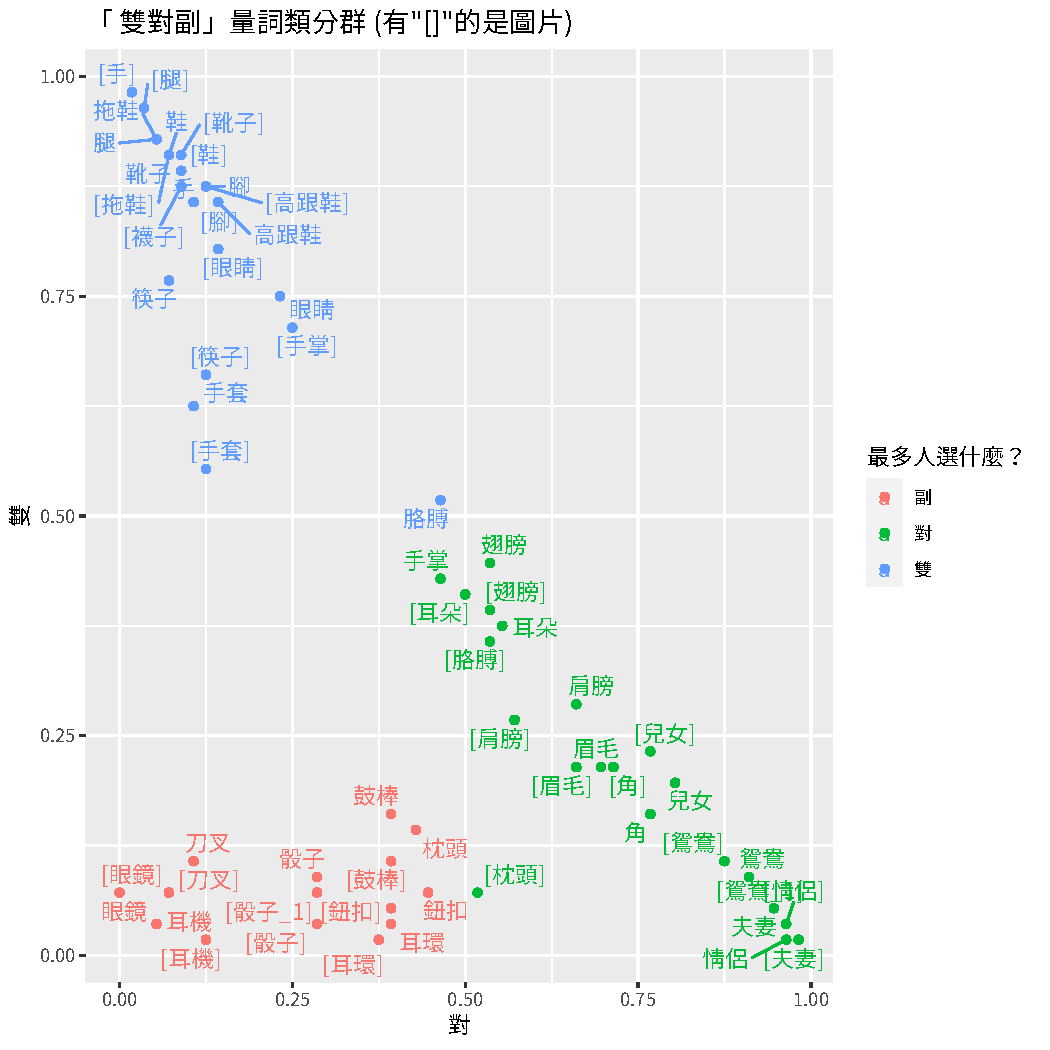
\includegraphics[width=1.2\textwidth]{../plot_1}
	\caption{「雙副對」量詞使用分佈}
	\label{two}
\end{figure}

\begin{figure}[h] %% 圖二
	\centering
	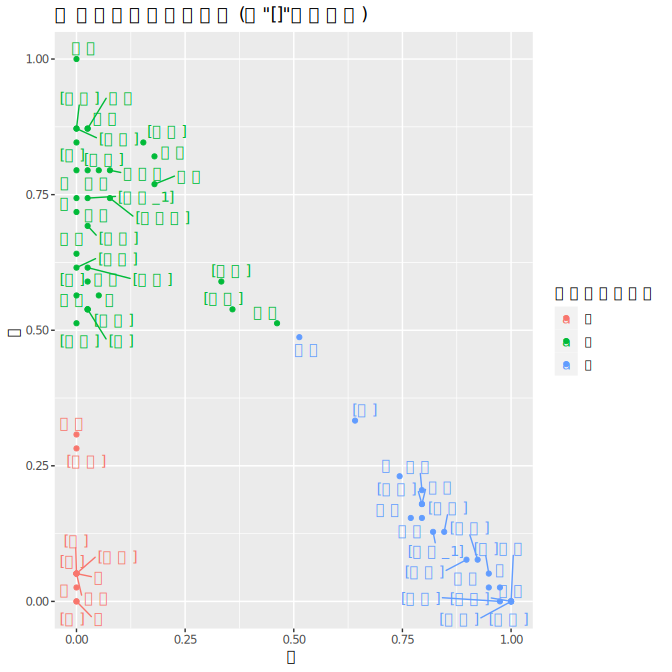
\includegraphics[width=1.2\textwidth]{../plot_2}
	\caption{「條根支」量詞使用分佈}
	\label{stick}
\end{figure}

\end{document}
